\chapter{\label{I_1}Le FRBR, modèle d'indexation conçu pour les bibliothèques} 


Cette partie s’attache à définir le \gls{FRBR} comme modèle de données adaptatif à différents items intégrés à un logiciel de gestion des collections. Si le FRFR est un modèle créé pour les items bibliographiques, il est également employé et adapté aux items de musée et aux archives audiovisuelles. Les collections d’archives audiovisuelles peuvent être modélisées par le \gls{FRBR} pour deux raisons. Leur statut hybride entre objet de collection et archives leur confère une complexité qui nécessite de modéliser leur description en niveaux. De plus, leur nature reproductible peut multiplier les versions, les publications, les exemplaires d’une même œuvre. La modélisation permet donc de rendre compte des liens entre les différents éléments d’une même œuvre. 


\section{\label{I_1_A}Un modèle conceptuel fondé sur les besoins utilisateurs}

La modélisation de données est structurante au sein d’un logiciel de gestion des collections, puisqu’elle désigne le “processus de création d’une représentation visuelle de l’ensemble d’un système d’information ou de parties de celui-ci pour communiquer les connexions entre les points de données et les structures."\footcite{2021d}. Le \gls{FRBR}, en tant que modèle de données, centralise l’expérience utilisateur au sein d’un outil de gestion des collections, lui permettant de visualiser les liens entre les contenus et de les localiser plus facilement.  Définissons plus en détail ce modèle de données dont la structure est déterminante pour notre étude sur l’implémentation de l’indexation automatique. 

Le FRBR, Functional Requirements for Bibliographic Records, est un modèle conceptuel de données bibliographiques élaboré par l'\gls{IFLA} (Fédération internationale des associations et institutions de bibliothèques) de 1992 à 1996. \footcite{zotero-item-651} Ce modèle établit la mise en place de quatre niveaux hiérarchiques pour le catalogage d'un document, comme le montre la figure \ref{figFRBR1}: le niveau Œuvre, niveau le plus haut décrivant les caractéristiques abstraites de la création l’œuvre, le niveau Expression, qui englobe les caractéristiques de son contenu intellectuel, le niveau Manifestation, qui décrit les modalités de sa publication, et finalement le niveau Item, qui décrit les caractéristiques individuelles du document en tant qu'exemplaire.  \footcite{zotero-item-651}  



\begin{figure}[htbp] 
	
	\centering 
	
	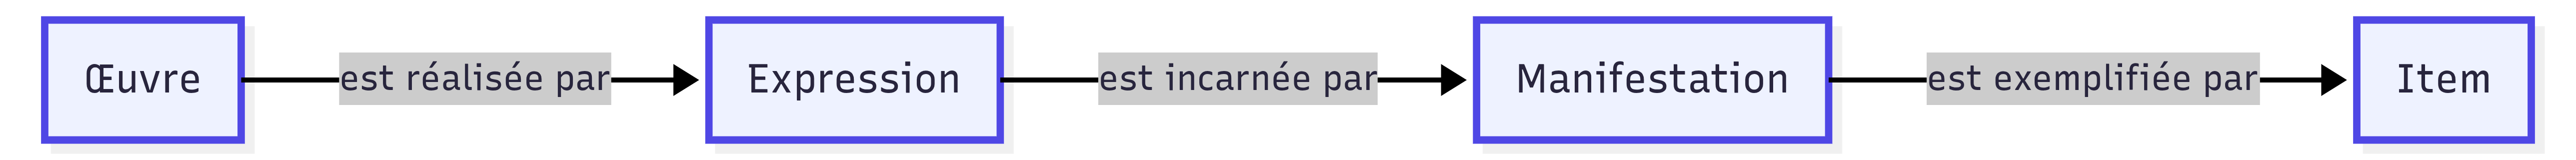
\includegraphics[width=1.0\textwidth]{images/FRBRfirstgroup.png} 
	
	\caption{Entités du modèle \gls{FRBR}} 
	
	\label{figFRBR1} 
	
\end{figure} 



Le \gls{FRBR} est qualifié de modèle entité-relation, qui modélise précisément les relations qui peuvent exister entre les différents niveaux de description et, de ce fait, entre les éléments d'un système d’information, afin de permettre à l'utilisateur de les retrouver plus facilement. Afin d’illustrer la manière dont s’articule la description d’un ouvrage bibliographique selon la modélisation proposée par le FRBR, prenons l'exemple de l'ouvrage \textit{Qu'est-ce que le cinéma} d'André Bazin. Au niveau Œuvre, est décrite l'idée intellectuelle de l'ouvrage, essentiellement matérialisée par son contexte de création. Cet ouvrage, est notamment exprimé et matérialisé au sein d'un texte intégral en quatre volumes écrit entre 1958 et 1962, dont les modalités sont décrites au niveau Expression. Cette expression de l’ouvrage est notamment publiée comme édition originale aux Editions du Cerf, dont les modalités sont décrites au niveau Manifestation. Enfin, l’exemplaire individuel de cette manifestation est potentiellement conservé dans une bibliothèque avec une côte unique, dont les caractéristiques physiques sont décrites au niveau Item. Une même œuvre peut être exprimée au sein de multiples expressions, de même qu’une expression peut faire l'objet de diverses manifestations. Le foisonnement d’éléments liés à une même œuvre peut rapidement rendre complexe la navigation de l’utilisateur au sein d’un outil de gestion des collections. La description proposée par le modèle \gls{FRBR} permet de distinguer les différentes étapes du cycle de vie d’une œuvre et ses différentes matérialisations, permettant ainsi une navigation plus fluide entre les éléments liés au sein d’un catalogue.  

Notons qu’à ces quatre entités de premier groupe Œuvre, Expression, Manifestation, Item), s'ajoutent deux entités de second groupe : Personnes et Collectivités. Elles expriment le rôle joué sur la production ou le contenu d'une ou plusieurs entités du premier groupe. \footcite{zotero-item-657} Par exemple, l'auteur est relié aux niveaux Œuvre et Expression, l'éditeur au niveau Manifestation, le catalogueur au niveau Item. 

Enfin, il existe des entités de troisième groupe intégrées au modèle, qui correspondent à des Concepts, Objets, Évènements ou Lieux liés aux entités de premier et de second groupe. \footcite{zotero-item-657} 

Réunies, les entités des trois groupes confondus modélisent une structure complexe caractérisée par les liens entre éléments, comme le montre la figure \ref{figFRBR2}  

\begin{figure}[htbp] 
	
	\centering 
	
	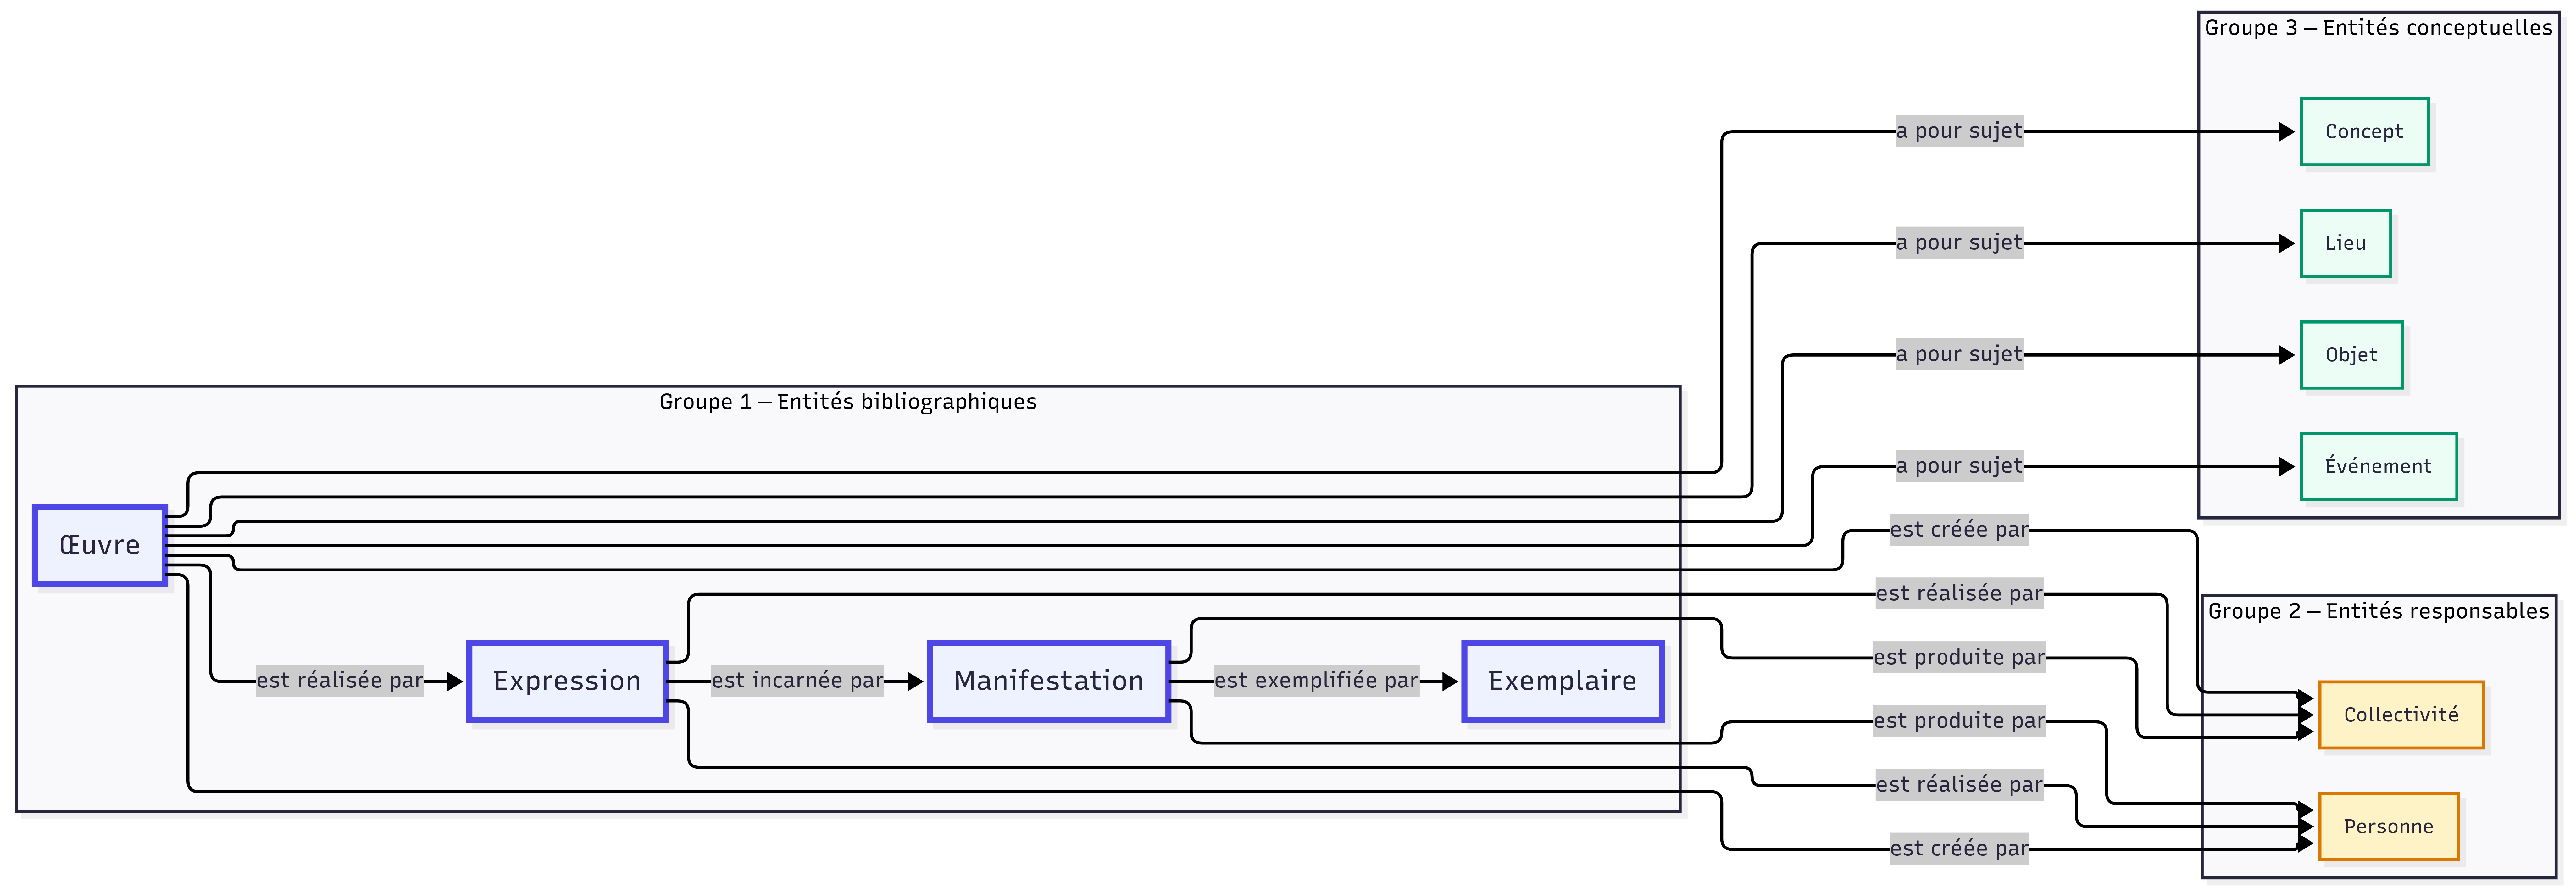
\includegraphics[width=1.0\textwidth]{images/FRBRentitesBiblio.png} 
	
	\caption{Entités du modèle FRBR} 
	
	\label{figFRBR2} 
	
\end{figure} 

Toutefois, dans le cadre de ce mémoire, nous nous concentrerons sur les entités de premier groupe, qui constituent les entités principales de description pour les archives audiovisuelles au sein du logiciel de gestion des collections créé par Skinsoft. Les entités de second et troisième groupe constituent moins des entités à part entière que des éléments de description contrôlés par des thésaurus.  

Le modèle \gls{FRBR}, fondé sur les relations entre entités, est avant tout conçu dans l’optique de faciliter la navigation de l'utilisateur au sein d'un catalogue, entre les liens qui régissent les différents éléments d'une collection.  Le \gls{FRBR} prétend en effet répondre à quatre besoins utilisateur principaux : trouver, identifier, sélectionner, obtenir. \footcite{zotero-item-653}. Il permet à l'utilisateur de localiser la ressource, d'identifier si elle correspond bien à ce qu'il cherche, de la sélectionner selon ses besoins, avant d'accéder finalement à son contenu. Nous ajouterons que le besoin fondateur de la création d'un tel modèle est également celui de pouvoir visualiser et explorer les liens de la ressource identifiée avec d'autres ressources pertinentes qui y sont directement associées. \footcite{zotero-item-653} Ce modèle de données se situerait donc à l'intersection de deux besoins principaux : celui d'améliorer la connaissance sur une ressource donnée en visibilisant ses relations, et celui d'améliorer l'expérience utilisateur en proposant une interface navigable et intuitive. 

%Donner un exemple d’institution qui utilise ce modèle et comment ça se matérialise dans un catalogue en ligne (bibliothèque kandinsky?) 

Notons que ces besoins s'appliquent non seulement à l'utilisateur faisant partie d'un public, au sein d'un catalogue ou d'une base de données en ligne, mais également à un utilisateur métier, interne à l'institution et gestionnaire des collections. C'est précisément sur les besoins métier de ce dernier que se concentre l'analyse de ce mémoire de recherche, puisque Skinsoft propose avant tout un outil de gestion des collections interne. De fait, les enjeux de l'implémentation et de l'adaptation du modèle \gls{FRBR} se situent au cœur des ambitions d'un logiciel de gestion des collections, dont l’objectif est d’améliorer l’interface afin d’assurer l’efficacité de l’utilisateur métier.  







%L'adoption de ces modèles dans les catalogues est réalisé dans l'objectif d'améliorer la visibilité des données au sein du web de données et donner accès au public aux données produites, même si ce mémoire se concentre sur l'utilisateur métier. (définir le web de données?) \footcite{zotero-item-661} 
\section{\label{I_1_B}Son adaptation à l'archivistique et au contexte muséal}

Le modèle \gls{FRBR} est un modèle conçu par et pour les bibliothèques. À ce jour, les bibliothèques n'utilisent plus seulement le modèle FRBR mais la somme du FRBR et de ses modèles étendus : le \gls{FRAD} (Fonctionnalités requises des données d'autorité) pour la description des autorités, et le FRSAD (Fonctionnalités requises des données d'autorité matière) pour la description des sujets.\footcite{zotero-item-651}. La somme de ces modèles constitue le modèle \gls{IFLA-LRM}, successeur du \gls{FRBR}. Le modèle \gls{FRBR} est toutefois largement utilisé dans le domaine de la gestion des collections muséales. Or, sa qualité de modèle ne prétend pas normaliser la description des données, seulement d’en cadrer l’affichage. De fait, les entités proposées par le modèle \gls{FRBR} peuvent paraître génériques, et doivent être soumises à une redéfinition à chaque implémentation selon le contexte donné \footcite{boeuf2008}. Cette flexibilité ne doit toutefois pas nuire à l'objectif principal, celui de faciliter la navigation de l'utilisateur, en explicitant les “interrelations" entres les notices et les données produites \footcite{boeuf2008}. Nous étudierons dans les chapitres suivants une double adaptation, celle du modèle \gls{FRBR} à d’autres types de documents : objets de collections et archives, et son adaptation à différents contextes institutionnels pour une même nature de documents, celle des archives audiovisuelles.  

%Analysons premièrement son adaptation au milieu archivistique. La difficulté principale de l'adaptation du modèle FRBR aux collections d'archives est que le niveau Œuvre ne peut contenir le plus haut niveau archivistique : le fonds d'archives. En effet, un fonds d'archive ne peut être considéré systématiquement comme une œuvre, puisque dans la plupart des cas, il s'agit plutôt d'une agrégation naturelle d'éléments quotidiens produits par une personne morale ou physique. Ainsi, un fonds d'archives ne peut être intégré à la définition d'une œuvre comme création intellectuelle et artistique distincte \footcite{fick2015}. Un fonds d'archives correspondrait davantage à un agrégat d'œuvres ou de travaux, niveau intermédiaire décrit par le modèle FRBR : "un ensemble de documents privés classés par des archives en un seul fonds"(traduction). \footcite{fick2015}. Le niveau manifestation est obsolète car les archives ne sont pas publiées ?  

%Développer un peu plus sur l’adaptation du modèle aux archives : qu’en est-il des autres niveaux ? À quoi ressemble un catalogue d’une institution qui utilise le FRBR pour les archives ? (À relier avec le sujet) 

Le modèle de données \gls{FRBR} a été adapté au milieu muséal à travers une version orientée objet, le \gls{FRBRoo}, extension du \gls{CIDOC-CRM} (object-oriented Conceptual Reference Model), l'ontologie de référence dédiée au patrimoine culturel et muséal \footcite{gillis2015}. Il s’agit d’un modèle conceptuel général visant l’interopérabilité entre les données provenant d’institutions diverses dont les musées, centres d’archives et bibliothèques.  

Ce dernier modélise une approche descriptive centrée sur les évènements entourant l’objet décrit. Ainsi, les entités bibliographiques ne sont plus seulement décrites par des attributs, mais par des évènements spatio-temporels qui les créent et les font évoluer selon différents contextes \footcite{dialogue2017} Cette adaptation du \gls{FRBR} est particulièrement pertinente pour la description de collections de musées composites et de différentes natures, pouvant englober à la fois la description de tableaux, sculptures, ouvrages, specimens, films, etc. Tandis que le \gls{FRBR} est modélisé à partir de la nature d’un document bibliographique le FRBRoo replace la description dans un contexte plus large, celui d’évènements situés dans l’espace et dans le temps, évènements qui peuvent agir sur n’importe quel type d’objet.  

Le \gls{FRBRoo} est un modèle intéressant pour la gestion des archives audiovisuelles. En effet, les \gls{Archivesaudiovisuelles} possèdent un statut hybride au sein d’institutions patrimoniales, relevant à la fois de la création artistique, de l’œuvre et d’un archivage du réel, d’un témoignage \footcite{zotero-item-669}. Le \gls{FRBRoo} propose deux entités pertinentes, qui pourraient permettre de distinguer l’évolution de ce double statut : l’œuvre (Individual work), et la captation ou l’enregistrement (Recording work). Par exemple, l’étape du tournage serait documentée par l’entité Captation ainsi que l'ensemble des évènements et des personnes qui y sont liés, alors que le montage serait documenté par l’entité Œuvre ainsi que les évènements et les personnes qui y sont liés. Le FRBRoo conserve ensuite les entités prévues par le FRBR : l’Expression, la Manifestation, l’Item.  

Néanmoins, si le FRBRoo constitue une adaptation pertinente du FRBR pour le milieu muséal, sa structure trop large ne permet pas de rendre compte la nature propre du médium cinématographique, qui fonde la gestion des collections audiovisuelles. Ainsi, les institutions préservatrices de collections audiovisuelles se tournent davantage vers des adaptations métier spécifiques, comme celle de la fédération des archives du film (FIAF). La FIAF propose en effet une application du FRBR spécifique aux usages métier de description des archives audiovisuelles, au sein d’un manuel de catalogage des images animées. 

\section{\label{I_1_C}Un modèle adapté aux archives audiovisuelles : le manuel de catalogage des images animées de la FIAF } 

L’adaptation du modèle FRBR aux archives audiovisuelles impose une double redéfinition : elle doit prendre en compte d’une part la nature propre du langage cinématographique, et d’autre part, les spécificités des corpus audiovisuels conservés. La modélisation en différentes couches de description prévue par le FRBR est pertinente pour le cinéma, qui partage avec le milieu bibliographique un mode de production industriel, permettant ainsi de distinguer la création intellectuelle de ses copies et diffusions multiples. Toutefois, les niveaux bibliographiques classiques dits WEMI (Work, Expression, Manifestation, Item) restent limitées pour la description métier des spécificités des archives audiovisuelles.  

Premièrement, alors que les bibliothèques conservent principalement des copies identiques d’une même publication, les archives d’images animées sont fréquemment amenées à gérer des objets uniques et rares tels que des \textit{rushes}, des films amateurs, montages inachevés, copies annotées, etc. \footcite{zotero-item-646}. Pour ce type de collections, le niveau Manifestation devient obsolète, en raison du caractère inédit de leur création. Deuxièmement, la distinction du FRBR bibliographique entre l’Œuvre (l’idée de création), et l’Expression (sa réalisation) s’adapte mal au contexte cinématographique. En effet, un film prend véritablement forme au moment du tournage puis du montage, rendant ainsi l’idée d’une existence abstraite de création en amont, caduque. Il parait alors plus pertinent d’appréhender l’œuvre cinématographique moins comme une entité abstraite en amont de son expression que comme une entité concrète ancrée dans un processus d’expression.  

Afin de répondre à ces contraintes imposées par le processus de création cinématographique, la FIAF a élaboré un manuel de catalogage des images animées \footcite{zotero-item-644}. Le manuel adapte le modèle FRBR en le combinant aux règles descriptives RDA (Ressources, Description, Accès) dédiées aux archives, et aux normes de description des œuvres cinématographiques (EN 15744 / EN 15907) \footcite{zotero-item-646}. Le manuel se focalise sur les entités de premier groupe afin d’en repenser l’articulation et de proposer de remplacer le schéma WEMI par le schéma WVMI (Work, Variant, Manifestation, Item).  

En effet la FIAF propose de fusionner le niveau Expression dans celui de l'Œuvre, permettant alors à l’Œuvre de regrouper la description intellectuelle et le processus de création de l’archive cinématographique. Par exemple, si nous prenons le film \textit{L'Aigle à deux têtes} (France, 1948, réalisé par Jean Cocteau), le niveau Oeuvre permettrait d’y décrire le contexte de création ainsi que le contenu. De plus, la FIAF propose une nouvelle entité, celle de Variante, optionnelle, qui se substitue à celle d’Expression. Elle permet de décrire toute version différente d’une œuvre originale dans la mesure où son sens principal n’est pas altéré. Par exemple, une version d’un film qui serait colorisée, censurée, doublée, remontée, etc. Si nous reprenons \textit{L'Aigle à deux têtes}, une variante possible est celle de la restauration du film en 4K en 2023, dont le niveau Variante permettrait de décrire les variations portées sur l’œuvre. La FIAF conserve par ailleurs le niveau de Manifestation, toutefois redéfini afin de pouvoir décrire la matérialisation physique ou numérique d’une Œuvre ou de sa Variante sur un support, ainsi que son contexte de diffusion. Par exemple, la manifestation de la version restaurée de \textit{L'Aigle à deux têtes} décrirait la sortie de cette version en Blu-Ray et DVD chez Rimini Editions. Enfin, le niveau Item est également conservé afin de décrire l’exemplaire physique ou le fichier numérique unique issu de la Manifestation d’une Œuvre ou de sa Variante. Cet exemplaire est concrètement préservé et géré par l’institution et décrit par des métadonnées de conservation.  

Cette restructuration du FRBR permet ainsi de répondre aux besoins métiers spécifiques de gestion de collections d’images animées. Selon la FIAF, la modélisation de cette réadaptation du FRBR au sein d’un outil de gestion des collections devrait permettre aux utilisateurs métier “d’identifier, sélectionner et acquérir” efficacement toutes les variantes d’une œuvre, l’ensemble des manifestations d’une version d’une œuvre, les exemplaires physiques disponibles d’une manifestation d’une œuvre \footcite{zotero-item-646}. La FIAF reprend ainsi les besoins utilisateurs fondateurs de la structuration du FRBR bibliographique en les adaptant à une nécessité de pouvoir circuler entre les différentes versions d’une œuvre à différents stades du processus de l’industrie cinématographique.  

Toutefois, l’implémentation d’un tel modèle au sein d’un outil de gestion des collections se heurte aux spécificités des différents corpus audiovisuels, dont certains ne possèdent pas de manifestation par exemple. En effet, si le modèle s'applique adéquatement aux corpus de cinéma dits "classiques" dont la chaîne de production industrielle est respectée : un film est réalisé à l'issue d'un tournage et d'un montage (Œuvre), puis distribué (Manifestation), et copié en multiples exemplaires (Item). Or, dans le cas de corpus spécifiques, expérimentaux, personnels, ou amateurs, qui font l’objet de descriptions complexes, la modélisation FRBR classique s'avère limitée. Ce type de corpus est notamment peu distribué ou diffusé, rendant notamment le niveau de Manifestation obsolète. 

Ainsi, le FRBR reste un modèle qu’il s’agit de réadapter à chaque contexte institutionnel \footcite{boeuf2008}. Le manuel de la FIAF agit comme un cadre théorique de structuration de la description pour la globalité des archives audiovisuelles, qui subit une redéfinition pour chaque type de corpus audiovisuel : amateur, commercial, documentaire, grand public, etc.  

Reproductibilité technique ? \footcite{zotero-item-669} 






		
		
		
		%le but ultime de la modélisation des données et de leur structuration est leur interopérabilité et leur versement sur le web de données par les institutions qui le souhaitent. Permet de passer de la donnée brute à l'information intelligible. dès l'inventaire des données, la modélisation doit être prise en compte et également le multilinguisime pour faciliter l'ouverture des données. \footcite{chambonnet} 
		
		%Nécessité d'uniformiser même si les corpus sont hétérogènes pour assurer l'intéropérabilité des données.  
		
		%Transition vers la deuxième sous partie : adapter le FRBR aux archives audiovisuelles 
		
		
		
		%à replacer - fin de la deuxième sous partie :  
		
		%Transition entre le modèle de données et l'automatisation :  
		
		%justification de la clarté du modèle FRBR pour la mise en place d'un modèle automatique :  
		
		% 
		
		%Impact de l'indexation automatique sur les données : 
		
		% 
		
		%"Comme le repérage d’entités visuelles demande énormément d’informations locales, les bases de données d’indexation constituées à partir de la reconnaissance des entités sont conséquentes (elles peuvent avoir une taille supérieure à celle des vidéos elles-mêmes) et font l’objet de recherches au sein de l’établissement pour en optimiser les temps de calcul. Dans ce contexte, la qualité et la modélisation des données jouent un rôle fondamental car c’est sur les bases de données que les algorithmes sont entrainés."\footcite{moiraghi2018} 
		
		% 
		
		%Nous prenons ici la pensée inverse, ce n'est pas seulement l'indexation automatique qui nécessite un modèle de données qualitatif, mais nous réfléchissons justement à la manière dont le modèle de données façonne l'indexation automatique et la manière dont l'indexation automatique permet de repenser le modèle de données dans lequel est implémentée.  
		
		% 

